\documentclass[twocolumn]{aastex631}

% Packages
\usepackage{microtype}  % ALWAYS!
\usepackage{amsmath}
\usepackage{amsfonts}
\usepackage{amssymb}
\usepackage{multirow}

\newcommand{\mlg}{M$_{\rm LG}$}
\definecolor{pink}{RGB}{232,132,161}
\newcommand{\kc}[1]{\textcolor{pink}{\textbf{#1}} }
\newcommand{\mud}{\mu_\delta}
\newcommand{\mua}{\mu_\alpha^*}
\newcommand{\bov}{\boldsymbol{v}}
\newcommand{\vel}[2]{\bov_{\rm #1 \to #2}}
\newcommand{\mwbary}{\rm MW_{bary}}
\newcommand{\mwdisk}{\rm MW_{disk}}

% Style tweaks
% \renewcommand{\twocolumngrid}{\onecolumngrid}
% \setlength{\parindent}{1.1\baselineskip}
% \sloppy\sloppypar\raggedbottom\frenchspacing


%%%%%%%%%%%%%%%%%%%%%%%%%%%%%%%%%%%%%%%%%%%%%%%%%%%%%%%%%%%%%%%%%%%%%%%%%%%%%%%%
\shorttitle{Updated Local Group Mass from Timing Argument}
\shortauthors{Chamberlain, Price-Whelan et al.}

%%%%%%%%%%%%%%%%%%%%%%%%%%%%%%%%%%%%%%%%%%%%%%%%%%%%%%%%%%%%%%%%%%%%%%%%%%%%%%%%
\graphicspath{{./}{figures/}}
% Missions
\newcommand{\project}[1]{\textsl{#1}}

% Packages / projects / programming
\newcommand{\package}[1]{\textsl{#1}}
\newcommand{\acronym}[1]{{\small{#1}}}
\newcommand{\github}{\package{GitHub}}
\newcommand{\python}{\package{Python}}
\newcommand{\astropy}{\package{Astropy}}

% Stats / probability
\newcommand{\given}{\,|\,}
\newcommand{\norm}{\mathcal{N}}
\newcommand{\pdf}{\textsl{pdf}}

% Maths
\newcommand{\dd}{\mathrm{d}}
\newcommand{\transpose}[1]{{#1}^{\mathsf{T}}}
\newcommand{\inverse}[1]{{#1}^{-1}}
\newcommand{\argmin}{\operatornamewithlimits{argmin}}
\newcommand{\mean}[1]{\left< #1 \right>}

% Non-scalar variables
\renewcommand{\vec}[1]{\ensuremath{\bs{#1}}}
\newcommand{\mat}[1]{\ensuremath{\mathbf{#1}}}

% Unit shortcuts
\newcommand{\Msun}{\ensuremath{\mathrm{M}_\odot}}
\newcommand{\Mjup}{\ensuremath{\mathrm{M}_{\mathrm{J}}}}
\newcommand{\kms}{\ensuremath{\mathrm{km}~\mathrm{s}^{-1}}}
\newcommand{\pc}{\ensuremath{\mathrm{pc}}}
\newcommand{\kpc}{\ensuremath{\mathrm{kpc}}}
\newcommand{\Mpc}{\ensuremath{\mathrm{Mpc}}}
\newcommand{\kmskpc}{\ensuremath{\mathrm{km}~\mathrm{s}^{-1}~\mathrm{kpc}^{-1}}}
\newcommand{\dayd}{\ensuremath{\mathrm{d}}}
\newcommand{\yr}{\ensuremath{\mathrm{yr}}}
\newcommand{\Kel}{\ensuremath{\mathrm{K}}}

% Misc.
\newcommand{\bs}[1]{\boldsymbol{#1}}

% Astronomy
\newcommand{\DM}{{\rm DM}}
\newcommand{\feh}{\ensuremath{{[{\rm Fe}/{\rm H}]}}}
\newcommand{\df}{\acronym{DF}}

% TO DO
\newcommand{\todo}[1]{{\color{red} TODO: #1}}
\newcommand{\apw]}[1]{{\color{green} APW says: #1}}

% Projects
\newcommand{\gaia}{\textsl{Gaia}}
\newcommand{\gaiadr}{\textsl{Gaia}~\acronym{EDR3}}


% Affiliations
\newcommand{\affuofa}{University of Arizona, 933 N. Cherry Ave,
    Tucson, AZ 85721, USA}
\newcommand{\affcca}{Center for Computational Astrophysics, Flatiron Institute,
    Simons Foundation, 162 Fifth Avenue, New York, NY 10010, USA}

%% This is the end of the preamble.  Indicate the beginning of the
%% manuscript itself with \begin{document}.

\begin{document} 

\title{
    A timing argument mass for the Local Group accounting for the
    Milky Way--LMC reflex motion
}

\author[0000-0001-8765-8670]{Katie~Chamberlain}
\affiliation{\affuofa}

\author[0000-0003-0872-7098]{Adrian~M.~Price-Whelan}
\affiliation{\affcca}

\author{Others!}


\begin{abstract}
    % \textbf{Context} 
    The Local Group mass sets the distribution and kinematics of its constituent galaxies and is necessary to place it in a cosmological context. Though challenging to measure, one method that has been used to estimate the Local Group mass is the Timing Argument, which constructs a Keplerian orbital model that is matched to the observed kinematics of M31 with respect to the Milky Way. 
    However, recent observations of stellar tracers in the outer MW halo have revealed an excess velocity dipole in the radial velocities that can be interpretted as a bulk motion of the Milky Way disk with respect to its outer halo. 
    This motion of the disk has previously been unaccounted for in Timing Argument models. 
    % \textbf{Aims} 
    We aim to infer a Local Group mass that accounts for the reflex motion of the Milky Way disk.    
    % \textbf{Methods} 
    We use Bayesian techniques to fit collected datasets of 6D phase-space information of M31 and determine the dependence of the inferred Local Group mass on the magnitude of the reflex motion.
    % \textbf{Results} 
    We provide an updated Local Group mass of $4.69\pm0.71 \times 10^{12}$M$_\odot$ assuming a disk travel velocity of $32\rm km/s$. 
    Additionally, we find that the inclusion of the reflex motion of the MW disk systematically lowers the inferred Local Group mass via the Timing Argument, and that the recovered mass depends strongly on the assumed travel velocity of the disk.
    Further measurements of the reflex motion of the disk will likely yield a larger observed travel velocity, and therefore a lower Local Group mass. In addition, improvements to proper motion measurements from future Gaia data releases may improve the constraint on the Local Group mass by a factor of $\sim2$.
    % \textbf{Conclusions}
    The Timing Argument remains one of the only ways to measure the Local Group mass independently of the masses of the individual component galaxies, but it is clear that the effect of the LMC must be accounted for when using these techniques. 

\end{abstract}

\section{Introduction}
\label{sec:intro}

\begin{itemize}
    \item importance of knowing mass of the local group
    \item ways to measure local group mass
    \item \begin{itemize}
            \item other tracers? 
            \item introduction of timing argument 
            \item what previous TA measurements of the local group mass have been
          \end{itemize}
    \item what's wrong with previous use of TA?
        \begin{itemize}
            \item the LMC is massive and pulling on the MW disk
            \item previous use of timing argument did not account for travel velocity of the disk
            \item we include the travel velocity of the disk
        \end{itemize}
    \item cosmological impact
        \begin{itemize}
            \item bias and calibration of the timing argument 
            \item what a lower/higher group mass means (we're gonna be more consistent w other group mass measurements, I think?)
        \end{itemize}
    \item\textbf{Par ?: The timing argument }
    
\end{itemize}

%%%%%%%%%%%%%%%%%%%%%%%%%%%%%%%%%%%%
\section{Methods}\label{sec:methods}
%%%%%%%%%%%%%%%%%%%%%%%%%%%%%%%%%%%%
We assumed a Keplerian model for the dynamics of the M31-MW system, accounting for the reflex motion of the Milky Way disk, and constrained the mass of the Local Group using observed kinematics of M31.  

\textbf{The dynamics of the M31-MW system can be approximated by simple Keplerian orbits.}
Local Group dynamics are dominated by the local gravitational potential where the Hubble flow can be neglected~\cite{}. We construct a Keplerian orbital model where the kinematics of the M31-MW system are completely determined by 4 model parameters: (\mlg, $a$, $e$, $\eta$) where \mlg is the mass of the Local Group, and $a$, $e$, and $\eta$ are the semi-major axis, eccentricity, and eccentric anomaly of an orbit of M31 about the MW. The analytic equations for the separation, the elapsed time since pericenter, and the velocity components from the equations of motion for a two body Keplerian interaction are:
\begin{equation}\label{eq:r}
  r = a(1-e\cos\eta)\\
\end{equation}

\begin{equation}\label{eq:t}
  t=\bigg(\frac{a^3}{GM}\bigg)^{1/2}(\eta-e\sin\eta)
\end{equation}

\begin{equation}\label{eq:vrad}
  v_{rad} = \bigg( \frac{a}{GM} \bigg)^{-1/2} \frac{e\sin\eta}{1-e\cos\eta}
\end{equation}

\begin{equation}\label{eq:vtan}
  v_{tan}= \bigg( \frac{a}{GM} \bigg)^{-1/2} \frac{\sqrt{1-e^2}}{1-e\cos\eta}.
\end{equation}
where, in our model, $r$ is the distance between the centers of mass of M31 and the Milky Way, $t$ is the time that has elapsed since the M31-MW was at pericenter, and $v_{rad}$ ($v_{tan}$) is the radial (tangential) velocity of M31 toward the MW. 

% info about coordinate system setup
\textbf{We choose a coordinate system centered on the disk of the MW, where positive x is along the line of sight between the MW disk and the center of M31's disk, and positive y is in the direction of the tangential motion of M31.} Thus, the velocity vector of M31 in this Keplerian coordinate system is $(v_x, v_y, v_z) =(v_{rad},v_{tan},0)$. 

\textbf{To compare our model predictions of the M31-MW system to the observed kinematics, we must translate these quantities into observables to constrain our model with observational data.}
We adopt the notation of~\cite{Penarrubia2016}, where $\vel{A}{B}$ represents the velocity vector of \textit{A} as measured in the reference frame of \textit{B}. With this notation, $\vel{A}{B}$=-$\vel{B}{A}$ and $\vel{A}{C}$=$\vel{A}{B}$+$\vel{B}{C}$. Thus, the velocity of M31 with respect to the center of mass of the MW can be represented by $\vel{M31}{MW}$. To convert this quantity to a heliocentric reference frame, 
\begin{equation}  
  \vel{M31}{\odot} = \vel{M31}{\mwbary}+\vel{\mwbary}{\odot}
\end{equation}
where $\vel{M31}{MW}$ is determined completely by the model parameters and thus $v_{rad}$ and $v_{tan}$, and 
$\vel{\mwbary}{\odot}$ is the velocity vector of the center of mass of the MW with respect to the Sun. 

\textbf{The recent pericentric passage of the LMC has imparted a velocity boost on the disk and inner regions of the dark matter halo and disk of the Milky Way.} This implies that, in addition to the velocity boost to transform from the center of the MW disk frame to the Sun, we must also include a velocity boost that accounts for the 
reflex motion of the MW disk with respect to the outer halo.

Thus, the observed velocity vector of M31 from the Galactic frame is given by:
\begin{equation}
  \vel{\mwbary}{\odot} = \vel{\mwbary}{\mwdisk} + \vel{\mwdisk}{\odot}
\end{equation}
% It is slightly more instructive to think of $\bov{\rm MW_{disk} \to MW_{bary}}=-\bov{\rm MW_{bary} \to MW_{disk}}$, as~\cite{Petersen2021}
where $\vel{\mwbary}{\mwdisk}$ is the velocity vector of the center of the MW halo that is moving with travel velocity $v_{rm travel}$ from the reference frame of the barycenter of the outer, unperturbed dark matter halo of the MW, and $\vel{\mwdisk}{\odot}$ is the standard transformation from the Galactocentric frame to the Galactic frame.
Then, $\vel{\odot}{\mwdisk}$ is the velocity vector of the Sun about the MW disk center, given by 
\begin{equation}
  \vel{\odot}{\mwdisk}=({\rm U}_\odot, {\rm V}_\odot + V_0, {\rm W}_\odot)  
\end{equation}



We used a No-U-Turn Sampler (NUTS) implemented with \texttt{pymc3}~\citep{Salvatier2016} to sample from the posterior distribution of model parameters \mlg, $a$, $e$, $\eta$, \kc{and $\alpha$, where $\alpha$ is a parameter that fixes the pole of the orbital plane of M31, and thus establishes the angle between the Keplerian tangential velocity and the proper motion measurements -- did we end up utilizing alpha?}. We set normal priors on the distance to M31 and the Local Group mass, a uniform prior on $\ln(1-e)$, and \kc{an angle prior implemented in the pymc3\_ext package, don't know how to describe this} (see Table~\ref{table:priors} for details). We ran our model with 1 chain for 4000 tuning steps and 2000 draws. 

% \begin{equation}
%   \mathcal{L}(| \boldsymbol{S})
% \end{equation}
% where $\boldsymbol{S} = ($\mlg$, a, e, \eta)$




\begin{table}
  \centering
  \begin{tabular}{lc}
  \hline\hline
  Prior  & Description \\\hline
  \mlg: $\mathcal{N}(4.5,3)\times10^{12}\Msun$ & Mass of the Local Group\\
  %  
  $r$: $\mathcal{N}(700,100)$kpc & Distance from M31 to $\mwdisk$\\
  %
  $\ln(1-e)$: $\mathcal{U}$(-10,0) & Eccentricity (close to 1) \\
  %
  $\eta$: angle(0,2$\pi$)& Eccentric anomaly\\
  \multirow{2}{*}{$\alpha$: angle(0,2$\pi$)} & Angle between M31 orbital\\
  & pole and Galactocentric\\
  \hline\hline
  \end{tabular}
  \caption{\label{table:priors}Priors \kc{note: on \mlg and $r$, we also set bounds? how should I show those here? or should they go in the text?}}
\end{table}




%%%%%%%%%%%%%%%%%%%%%%%%%%%%%%%%%%%
\section{Datasets}
%%%%%%%%%%%%%%%%%%%%%%%%%%%%%%%%%%%
We use heliocentric radial velocities and proper motions. 

See~\ref{table:data} for values.
\begin{table}
  \centering
  \begin{tabular}{lc|c}
    \hline\hline
                    & Dataset 1                     & Dataset 2 \\\hline
  $D$               &  770 $\pm$ 40 \rm kpc\cite{}     &           \\
  $v_{\rm rad}$     &           &           \\
  $\mu_\alpha^*$    & 44.6$\pm$12.66\cite{} \\
  $\mu_\delta$      & -32.1$\pm$12.21 $\mu\rm as/yr$ & \\
  (U$_{\rm pec}$, V$_{\rm pec}$, W$_{\rm pec}$) & (11.1, 12.24, 7.25)& \\
  V$_0$             & 239.3$\pm$10.3 km/s & \\
  %              &           &           \\
  %              &           &           \\ 
  \hline\hline
  
  \end{tabular}
  \caption{\label{table:data}Observational datasets used for comparison throughout analysis.}
\end{table}

% \footnote{note: Dataset 1 values of the proper motions are given as ($v_{w}, v_{N}$), then $(\mu_\alpha^*, \mu_\delta)$ were derived given $v_W=-\mua D$ and $v_N=\mud D$}

%%% Schematic %%%
\begin{figure*}[htb]
    \centering
    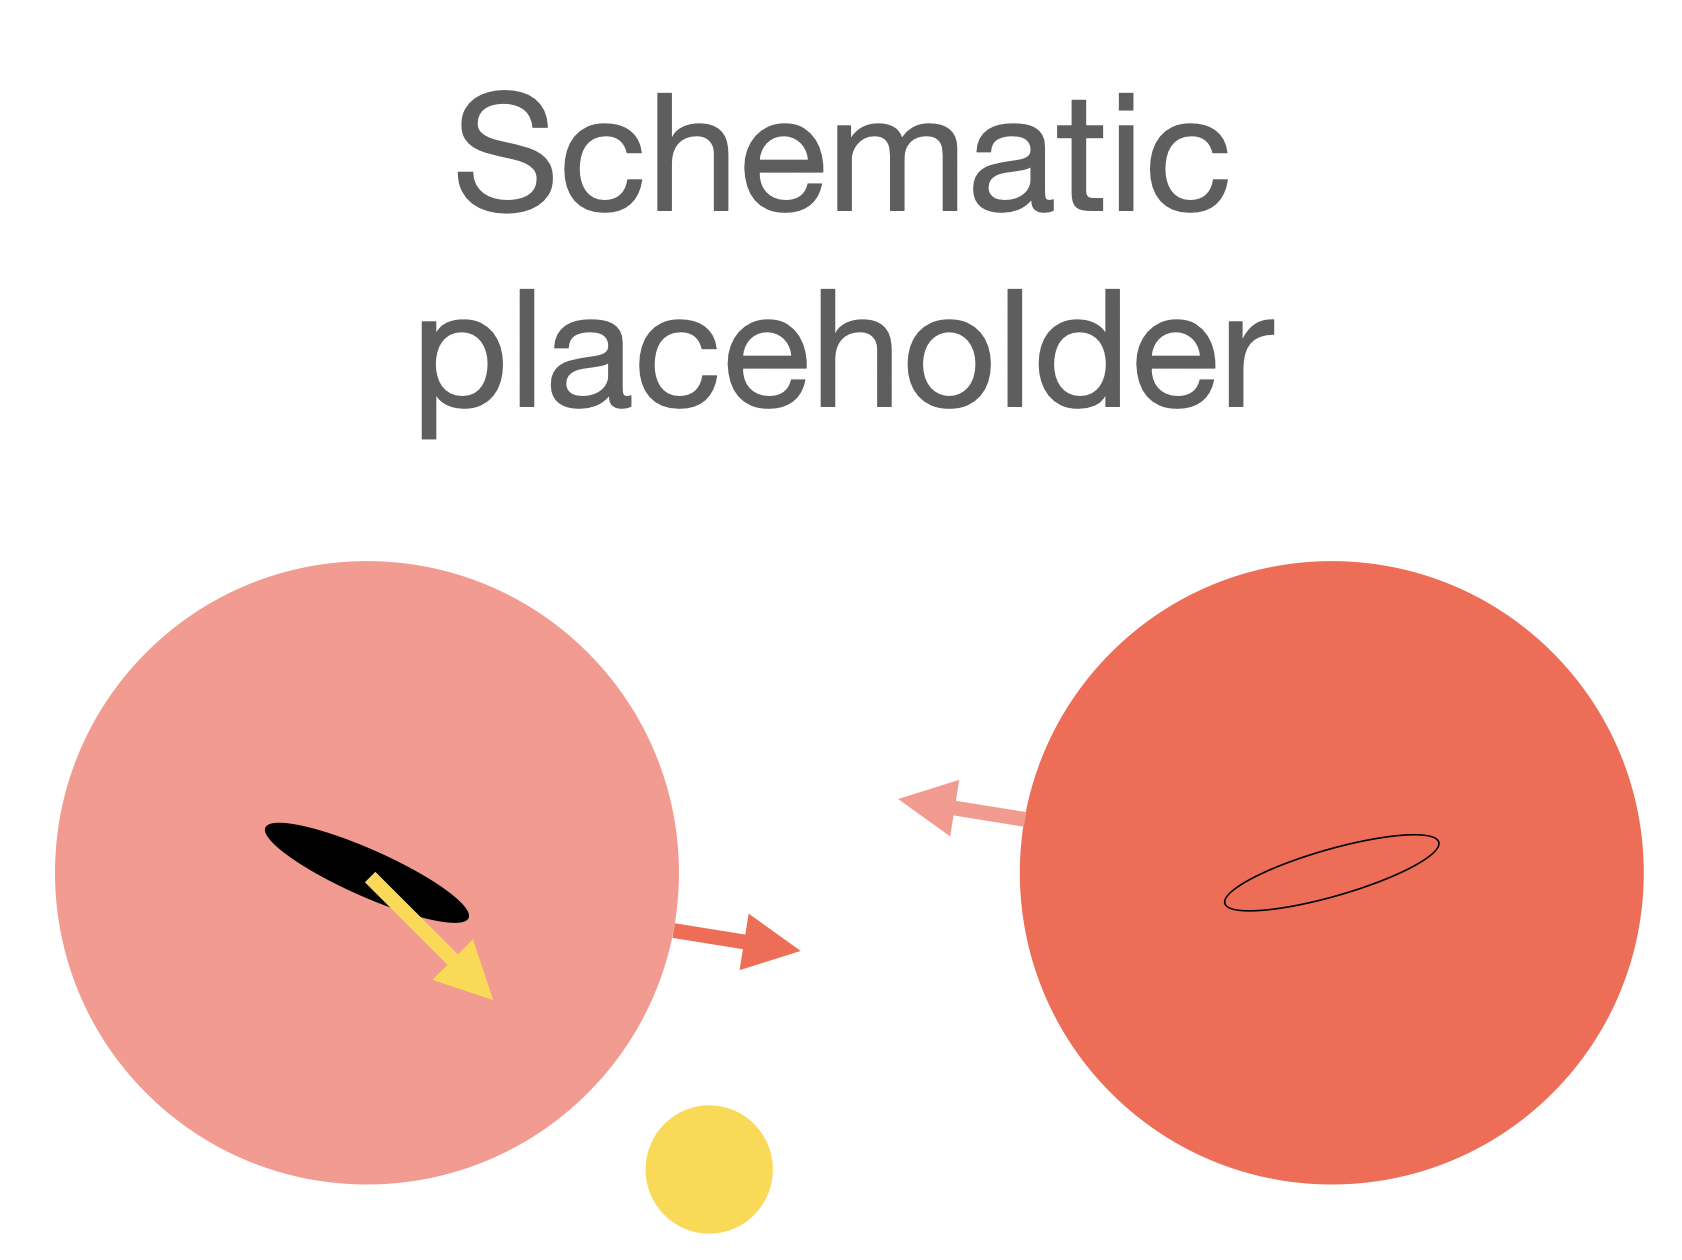
\includegraphics[width=0.8\columnwidth]{schematic_placeholder.png}
    \caption{\label{fig:schematic} Placeholder for whatever schematic we're going to end up creating
    }
  \end{figure*}

\kc{need tables with the data values and referencces for the observables used to constrain our model}

%%%%%%%%%%%%%%%%%%%%%%%%%%%%%%%%%%%
\section{Results: Local group mass estimates}
%%%%%%%%%%%%%%%%%%%%%%%%%%%%%%%%%%%
\label{sec:results}
We used a Bayesian model to place constraints on the mass of the Local Group and the distance between M31 and the Sun using the Timing Argument. Our model of the Local Group includes the reflex motion of the Milky Way disk and results in new constrains on the mass of the Local Group to 4.69$\pm0.71 \times 10^{12}\Msun$. This mass is lower than reported by~\cite{vdm2012} ($4.93\pm 1.63\times 10^{12}\Msun$) though significantly higher than~\cite{Penarrubia2016} ($\sim2.64\pm0.4\times 10^{12}\Msun$).

We found that, for both considered datasets, our model prefers lower Local Group masses and a lower eccentricity orbit compared to models that do not include MW disk reflex motion. Fig.~\ref{fig:contour} shows the 95\% contours from the sampled posterior PDFs of the distance to M31, the eccentricity of the orbit of M31 with a fixed MW, and the inferred Local Group mass. Arrows in the bottom left panel of the corner plot indicate the shift to lower masses and eccentricities when introducing the reflex motion of the MW. 

The direction of the motion of the disk is directly tied to the behavior of the inferred mass of the Local Group.In this case, the orbit of the LMC and location of the LMC at pericenter are in the same region of the sky as M31 such that the radial component of motion is in the direction of M31. Thus, the observed radial velocity of M31 will be higher than for an unperturbed MW halo. Since $-v_{rad}\propto M^{1/2}$ for an infalling system, a smaller (but still negative) radial velocity will yield a lower Local Group mass. 

The eccentricity decreases significantly for Dataset 2 compared to Dataset 1. This is primarily due to the larger measured proper motions of Dataset 2. \kc{Why does e decrease with our model? disk motion must be somewhat tangential to the proper motion of andromeda? }

Constraints on the distance to M31 remain roughly unchanged for both datasets, primarily because our model does not introduce a physical displacement of the MW disk, since we assume the motion of the disk over the past XX years since the LMC achieved pericenter is negligible compared to the separation between M31 and the MW. Thus, the inclusion of the reflex motion of the disk in our model does not affect constraints on the distance to M31. 


\kc{Why are we interested in local group mass as a function of travel vel and why did we test it?}
\begin{itemize}
  \item The observed travel velocity can change as a function of the distance of tracers, thus it's likely that the current measurements on $v_{travel}$ of 32km/s are just a lower bound on the actual reflex motion of the disk. 
\end{itemize}
\kc{What did we find Fig.~\ref{fig:mvsv}?}
\begin{itemize}
  \item 
\end{itemize}
\kc{What does this mean? - should this be in discussion instead? }

\kc{Why are we interested in pm error improvement and why did we test it?}
\kc{What did we find about the pm improvements Fig.~\ref{fig:mvspm}?}
\kc{What does this mean? - should this be in discussion instead? }


\begin{figure*}[htb]
  \centering
  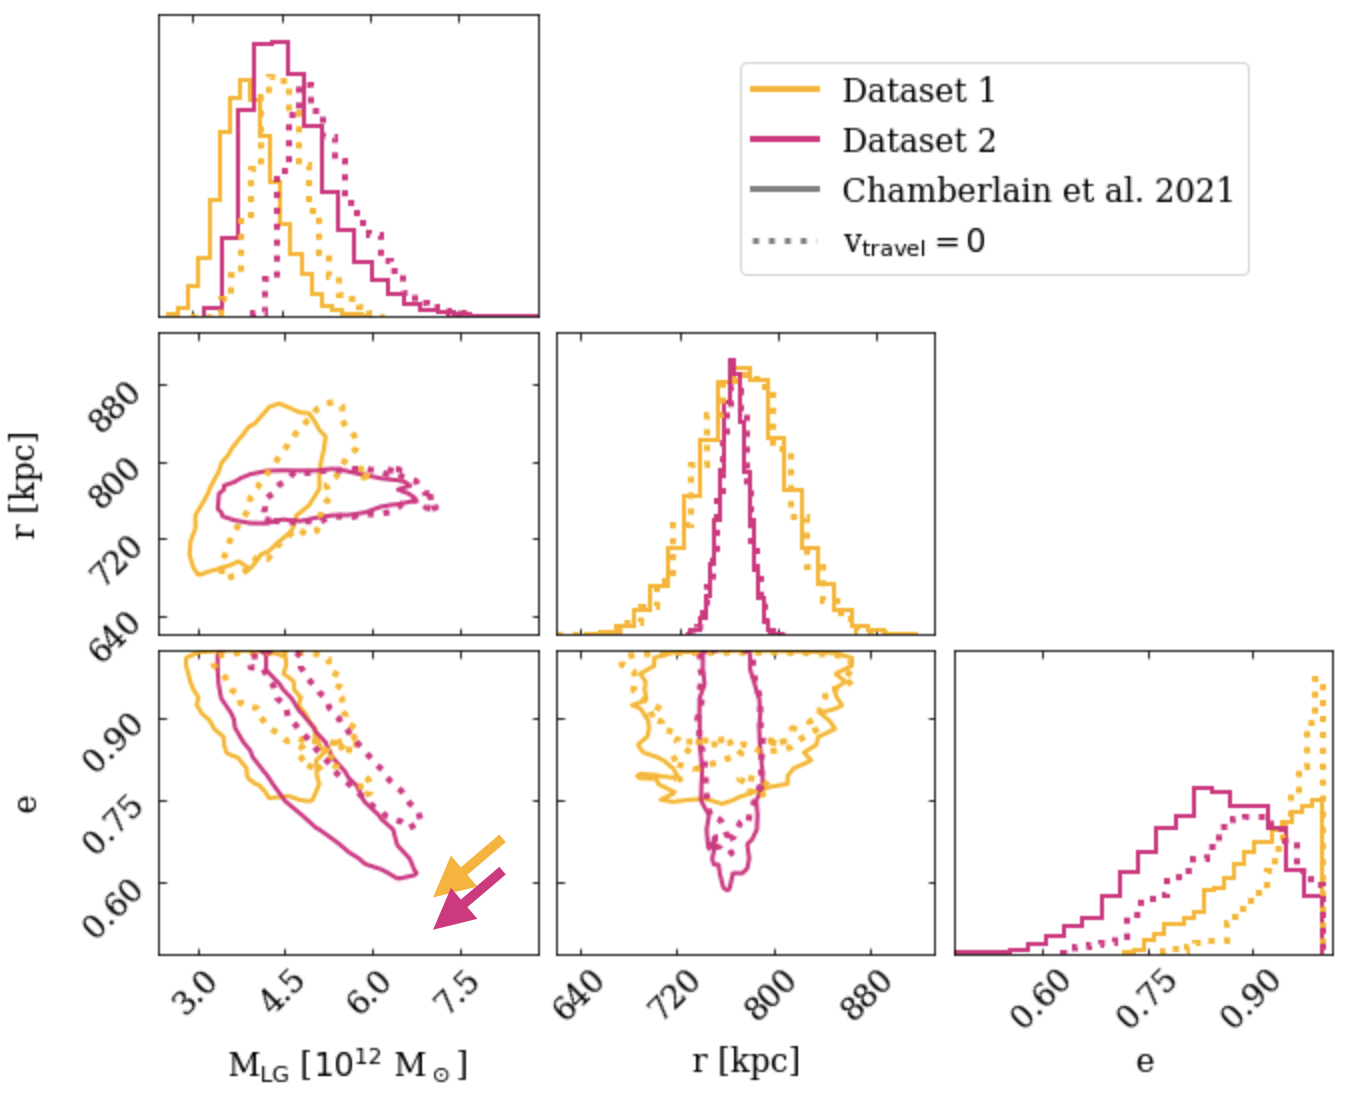
\includegraphics[width=0.8\textwidth]{analyze-runs-contour-arrows.png}
  \caption{\label{fig:contour} 95\% contours of sampled posterior distributions for two observational datasets (pink and yellow) of a subset of our model parameters: the total mass of the Local Group (\mlg), the distance between the Sun and M31 ($r$), and the eccentricity of the orbit of M31 about a fixed MW ($e$). A stationary MW disk is shown in the dotted contours, while our model, which includes the reflex motion of the MW disk, is shown in solid lines.  
  The distributions for the separations are unchanged between models, as our model does not implement a spatial shift to the location of the MW disk. A comparison between the two models shows that \textbf{the inclusion of the reflex motion of the MW disk systematically lowers the inferred mass of the Local Group} regardless of observational dataset. See text for discussion on the effects on eccentricity.
  \kc{should I change this plot to have color represent our model and grey be no travel velocity?, also should I only include 2 sets of contours (68 and 95) instead of just 95? also not rn this is a bad quality screenshot but didn't know how to put arrows on the figure w matplotlib because it's using subplots as part of \texttt{corner}}  }
\end{figure*}

\begin{figure}[htb]
    \centering
    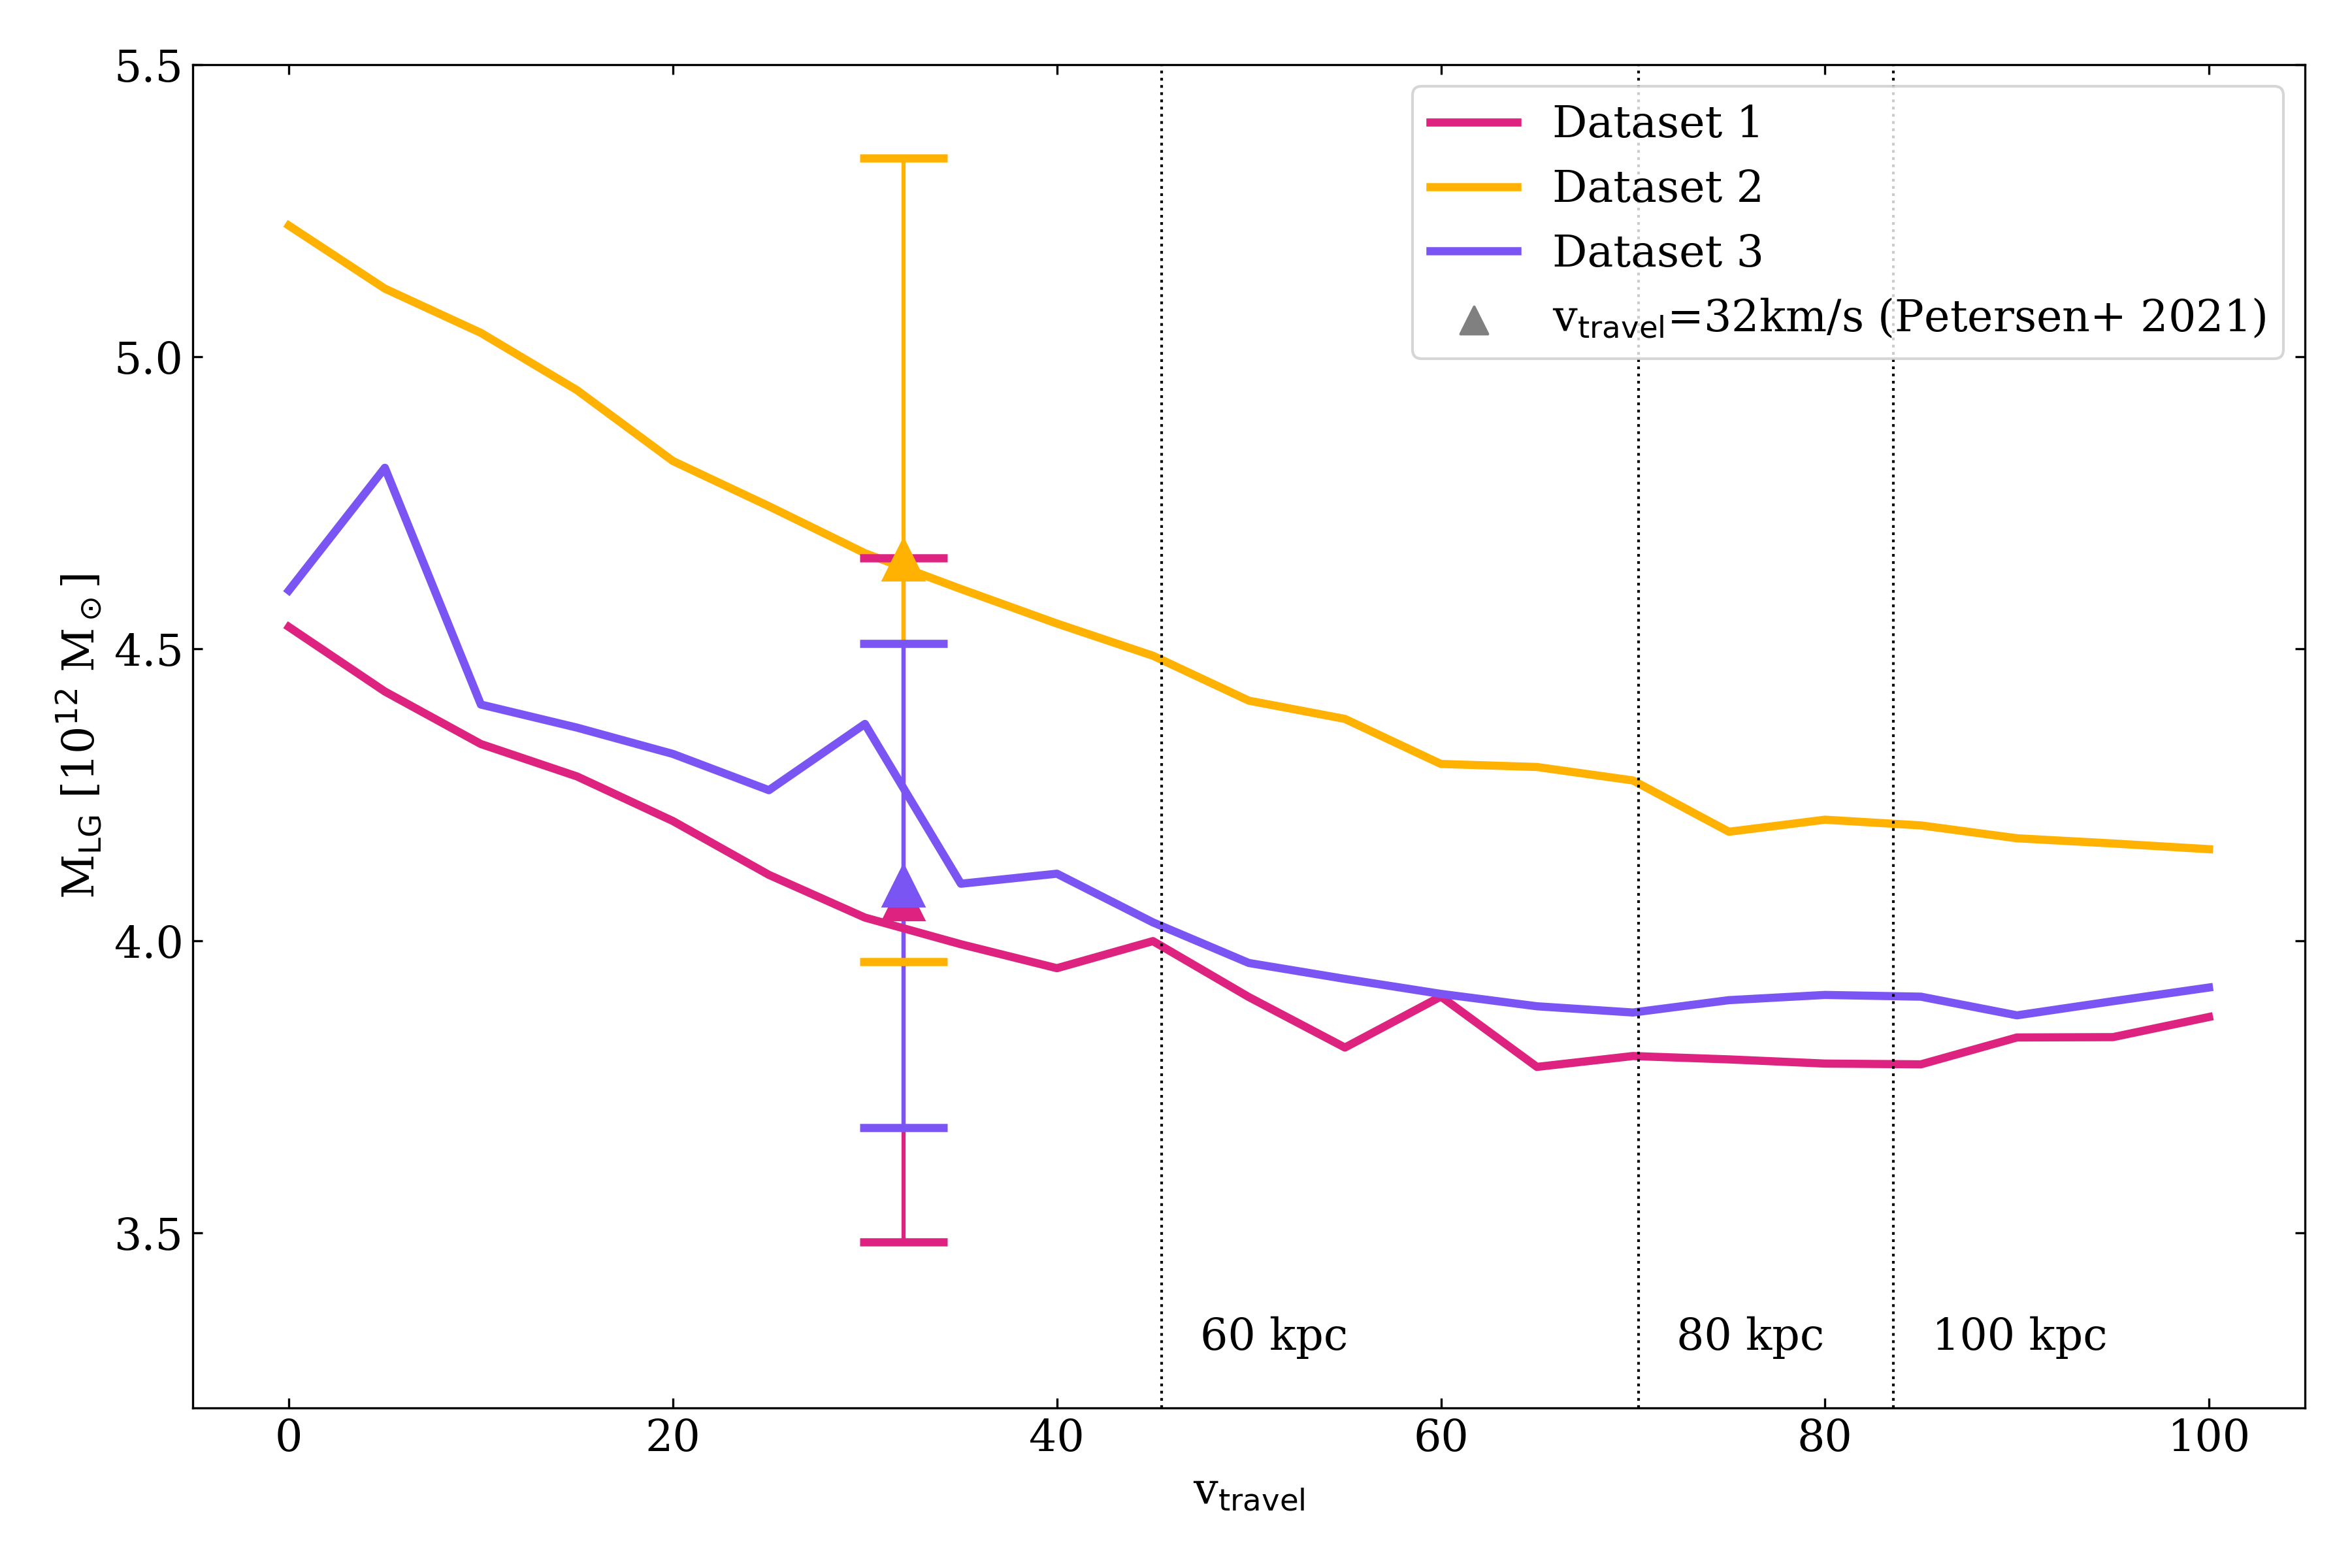
\includegraphics[width=\columnwidth]{analyze-runs-MvV.png}
    \caption{\label{fig:mvsv} Mean inferred Local Group mass as a function of travel velocity magnitude of the MW disk. Dataset 1 (yellow) yields masses that are systematically lower than Dataset 2 (pink), though they display the same general trends with increasing travel velocity. 
    The mean Local Group mass corresponding to the observed travel velocity from~\cite{Petersen2021} of 32km/s by the triangle points, including the 1-$\sigma$ spread on the mass at that travel velocity. \textbf{As the travel velocity of the Milky Way disk increases, the inferred Local Group mass decreases} before leveling off around 80km/s. 
     \kc{add vertical lines with vtravel predictions from different tracer distances. also... do we know why this levels off?}
    }
  \end{figure}

\begin{figure}[htb]
    \centering
    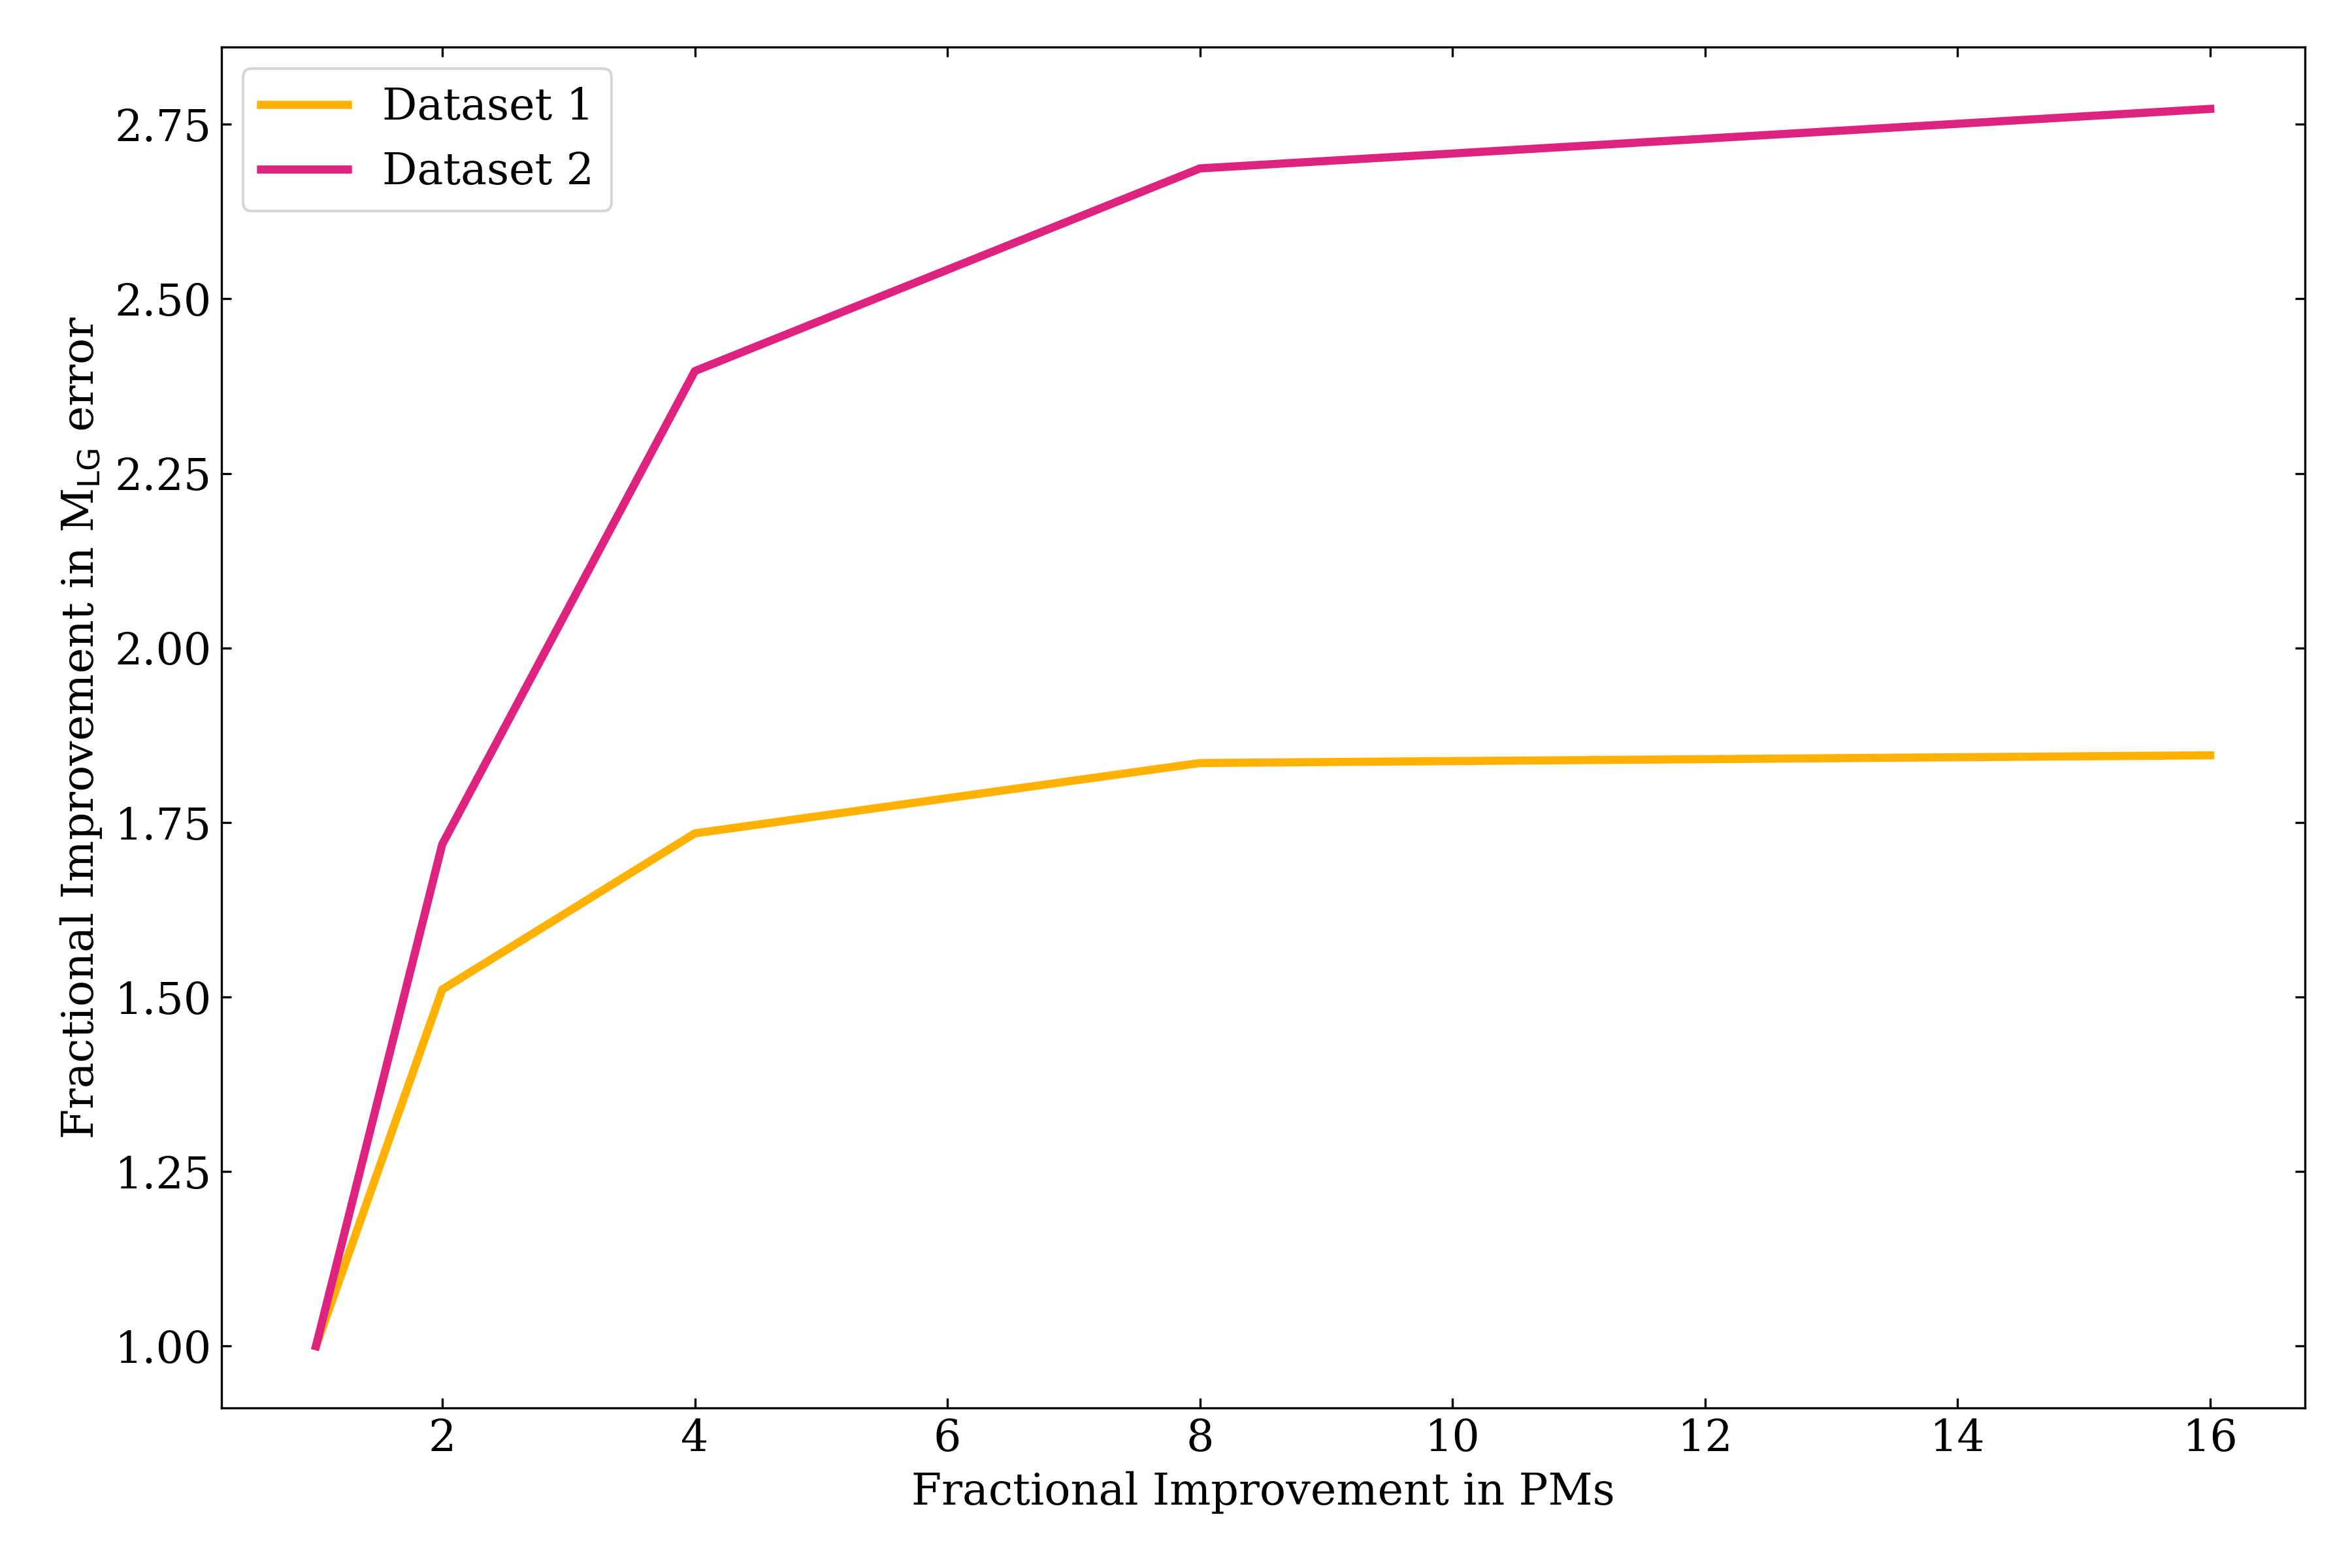
\includegraphics[width=\columnwidth]{analyze-runs-deltaMvsPM.png}
    \caption{\label{fig:mvspm} Improvement in the inferred Local Group mass as a function of fractional improvement in proper motion errors. The standard deviation in the mass decreases with decreasing proper motion error, and in particular, decrease by a factor of $\sim2.5$ for PMs that are 4 times smaller than in Dataset 2. \textbf{As future \textit{Gaia} data releases provide improved proper motion errors, constraints on the Local Group mass from the Timing Argument can improve by a factor of $>$2.} \kc{maybe remake this plot as fractional change in the error bar of the mass?}
    }
\end{figure}


%%%%%%%%%%%%%%%%%%%%%%%%%%%%%%%%%%%
\section{Comparison to M33--M31 system}
%%%%%%%%%%%%%%%%%%%%%%%%%%%%%%%%%%%

%%%%%%%%%%%%%%%%%%%%%%%%%%%%%%%%%%%
\section{Summary and Discussion}
%%%%%%%%%%%%%%%%%%%%%%%%%%%%%%%%%%%
\label{sec:discussion}


% \software{
%     Astropy \citep{astropy, astropy:2018},
%     gala \citep{gala},
%     IPython \citep{ipython},
%     numpy \citep{numpy},
%     pymc3 \citep{Salvatier2016},
%     scipy \citep{scipy}
% }
\appendix
\section{Todo:}
Does Katie get a CCA affiliation or no?

\bibliography{refs}{}
\bibliographystyle{aasjournal}

\end{document}
